%\documentclass[10pt,flushrt,preprint]{aastex}

\documentclass[preprint2]{aastex}

\usepackage{graphicx}
\usepackage[space]{grffile}
\usepackage{latexsym}
\usepackage{amsfonts,amsmath,amssymb}
\usepackage{url}
\usepackage[utf8]{inputenc}
\usepackage{fancyref}
\usepackage{hyperref}
\hypersetup{colorlinks=false,pdfborder={0 0 0},}
\usepackage{textcomp}
\usepackage{longtable}
\usepackage{multirow,booktabs}

\usepackage{natbib}

\newcommand{\truncateit}[1]{\truncate{0.8\textwidth}{#1}}
\newcommand{\scititle}[1]{\title[\truncateit{#1}]{#1}}


%% preprint2 produces a double-column, single-spaced document:

%% \documentclass[preprint2]{aastex}

%% Sometimes a paper's abstract is too long to fit on the
%% title page in preprint2 mode. When that is the case,
%% use the longabstract style option.

%% \documentclass[preprint2,longabstract]{aastex}

%% If you want to create your own macros, you can do so
%% using \newcommand. Your macros should appear before
%% the \begin{document} command.
%%
%% If you are submitting to a journal that translates manuscripts
%% into SGML, you need to follow certain guidelines when preparing
%% your macros. See the AASTeX v5.x Author Guide
%% for information.


%% You can insert a short comment on the title page using the command below.

\slugcomment{To appear in The Astrophysical Journal (ApJ)}

%% If you wish, you may supply running head information, although
%% this information may be modified by the editorial offices.
%% The left head contains a list of authors,
%% usually a maximum of three (otherwise use et al.).  The right
%% head is a modified title of up to roughly 44 characters.
%% Running heads will not print in the manuscript style.

\shorttitle{The Murchison Widefield Array Epoch of Reionization Pipelines}
\shortauthors{Danny Jacobs}

%% This is the end of the preamble.  Indicate the beginning of the
%% paper itself with \begin{document}.

\begin{document}

%% LaTeX will automatically break titles if they run longer than
%% one line. However, you may use \\ to force a line break if
%% you desire.

\title{The Murchison Widefield Array Epoch of Reionization Pipelines}

%% Use \author, \affil, and the \and command to format
%% author and affiliation information.
%% Note that \email has replaced the old \authoremail command
%% from AASTeX v4.0. You can use \email to mark an email address
%% anywhere in the paper, not just in the front matter.
%% As in the title, use \\ to force line breaks.

\author{
Danny Jacobs\altaffilmark{1},
Ian Sullivan \altaffilmark{2}
Bryna Hazelton \altaffilmark{2},
Bart Pindor \altaffilmark{3},
Cath Trott \altaffilmark{4},
Josh Dillon \altaffilmark{5},
Abraham Neben \altaffilmark{5},
Adam Beardsley \altaffilmark{2},
EoR list,
Builders list
}
\altaffiltext{1}{School of Earth and Space Exploration, Arizona State U., Tempe, AZ}
\altaffiltext{2}{Physics Dept. University of Washington, Seattle, WA}
\altaffiltext{3}{Melbourne University, Melbourne, Aus}
\altaffiltext{4}{Curtin University, Perth, Aus}
\altaffiltext{5}{Massachusetts Institute of Technology, Boston, MA}
\begin{abstract}
The Murchison Widefield Array (MWA) in Western Australia is currently
performing thousand hour integrations in the 2~m radio band with the
goal of detecting redshifted 21~cm emission from the Epoch of
Reionization (EoR) when the first stars are expected to reionize the
universe on cosmological scales. Our goal is to observe the power
spectrum of inter-galactic hydrogen as reionization proceeds and
constrain the timing and speed of this key step in the universe's
development. Because deep 21~cm power spectrum observations are very new
and require unprecedented levels of precision and foreground removal, we
have developed multiple analysis pipelines with redundant cross-checking
at each major processing stage to increase our confidence in the
reliability of the analysis. In this paper we describe the two parallel
analysis pipelines that will be used to analyze the MWA EoR data and
present initial power spectra and quality checks from the first nights
of EoR observing with the full MWA instrument.

\end{abstract}




%% Keywords should appear after the \end{abstract} command. The uncommented
%% example has been keyed in ApJ style. See the instructions to authors
%% for the journal to which you are submitting your paper to determine
%% what keyword punctuation is appropriate.

%\keywords{globular clusters: general --- globular clusters: individual(NGC 6397, NGC 6624, NGC 7078, Terzan 8}

\bibliographystyle{apj_w_etal}


\section{Introduction} 
  Study of intergalactic Hydrogen  in the early universe via the 21\,cm line is forecast to provide a wealth of astrophysical and cosmological information.  The 21\,cm line is both optically thin and spectrally narrow, making possible full tomographic reconstruction. Cosmological Hydrogen, which makes up 3/4 of baryonic matter, is neutral over cosmic time from recombination until reionized by the first batch of UV emitters (stars and accretion disks).  Reviews of 21 cm cosmology, astrophysics and observing can be found in \cite{Morales:2010p8093,Furlanetto:2006p2267,Pritchard:2012p9555,zaroubi2013epoch}.
  
Direct detection of HI during the Epoch of Reionization (cosmological redshifts $5<z<13$) is currently the goal of several new radio arrays. The LOw Frequency ARray \citep[LOFAR;]{Yatawatta:2013p9699}, the Donald C. Backer Precision Array for Probing the Epoch of Reionization (PAPER; \citet{Parsons:2014p10499}) and the Murchison Widefield Array (MWA; ) are all currently conducting long observing campaigns.

The analysis of the resulting data presents several challenges. The signal is faint; initial detection is being sought in the power spectrum with thousands of hours (multiple seasons) of integration required. This faint spectral line signal sits atop a continuum foreground four orders of magnitude brighter. At the same time, the instruments are the first of a new breed; fully correlated phased arrays with wide fields of view that strain the conventional assumptions of radio astronomy practice. The methods used to arrive at a well calibrated, foreground-free, estimation of the power spectrum are all new in the sense of the algorithms as well as the implementation.  

Given the challenges of using newly invented methods to reduce data from a novel instrument to make a low sensitivity detection, it is reasonable to consider the question of how one knows one is getting the ``right'' answer.  One option is to generate, as accurately as possible, a detailed simulation of the interferometer output. Full instrument simulation is computationally demanding and difficult to divorce from the analysis methods being tested, which at their core are instrument simulation engines. Development of an completely independent instrumental simulation and is the subject of ongoing work (see e.g. Nithyanandan et al. 2014), but is not available at scale at this time.  The second option is more pragmatic; compare the results of multiple independent pipelines.  Within the MWA collaboration efforts have centered around two, completely independent, paths from raw data to a power spectrum.  In this paper we outline each method, leaving the detailed descriptions to other papers, and demonstrate a comparison of both images and power spectra. 


The path from observation to power spectrum can be roughly divided into two parts: removal of foregrounds and estimation of power spectrum.\footnote{While statistical measures  such as \citet{Barkana:2008p2154} have also been proposed we choose the power spectrum for our initial analysis because the interferometer naturally measures in the Fourier plane.}  Recently two sorts of foreground removal have been suggested. Blind filtering, such as the delay/fringe-rate filtering approach \cite{Parsons:2012p8896,Liu:2014p10462,Liu:2014p10463},  which has been applied to data from the PAPER telescope \cite{Parsons:2014p10499}, applies a small amount of knowledge about the instrument to filter modes likely to be contaminated.  This method is comparatively robust in the face of uncertainty about the instrument and the sky. Meanwhile,  full forward modeling and subtraction of sky model such as that implemented by LOFAR (see e.g. \cite{Jelic:2008p2130,Yatawatta:2013p9699}), requires a much higher fidelity model of the instrument and the sky \citep{Datta:2010p8781,Vedantham:2012p10297}. If successful, this latter approach has the benefit of opening the most sensitive power spectrum modes and substantially improving the ability of early measurements to distinguish between reionization models \cite{Beardsley:2013p9952,Pober:2014p10390}. Recent work towards the goal of foreground subtraction includes better algorithmic handling of wide field imaging effects \cite{Tasse:2012p9459,Bhatnagar..2013ApJ,Sullivan:2012p9457,Ord:2010p8442}, continually improving catalogs of sky emission \citep{deOliveiraCosta:2008p2242,Jacobs:2011p8438}. Ongoing operation of the next generation low frequency arrays --LOFAR, PAPER and MWA are all in their second or third year of operation-- continues to push the refinement instrumental models and improve the accuracy of model subtraction.  Surveys of 21\,cm reionization foregrounds are currently under way. These include the MWA GLEAM\footnote{GLEAM: Galactic and Extragalactic All-sky MWA} survey  and the LOFAR MSSS\footnote{MSSS: Multi-frequency Snapshot Sky Survey}.   %todo insert MWACS cite when available

Within the MWA reionization pipelines foreground removal is handled either by Full Holographic Deconvolution \citep[FHD]{Sullivan:2012p9457} or the Real Time System \citep[RTS]{Ord:2010p8442}.  Here we use FHD to refer to a specific implementation of the algorithm constructed primarily for the reduction of MWA data, though it has been successfully applied to data from other telescopes.  The RTS is a hardware/software solution, originally designed to support operation of online imaging of the 512 element MWA, that has been repurposed and expanded into a general imaging package suitable for offline data reduction.


 Estimation of the power spectrum that takes into account instrumental and sky uncertainty can also ameliorate some of the conflict between foreground and background.  Work on these fronts has focused on improving the propagation of instrumental errors (EPPSILON\footnote{EPPSILON:Error Propagated Power Spectrum with InterLeaved Observed Noise}) and on better understanding the mathematical basis for estimating the power spectrum (CHiPS\footnote{Cosmological HI Power Spectrum}).  
 
 EPPSILON operates on residual images and is optimized for speed and error propagation. In simulation, the EPPSILON$+$FHD combination has uncovered new mode-mixing features in the foreground power spectrum \citep{Morales:2012p8790}.  Trott et al have implemented CHIPS which uses an optimal estimator approach (e.g. \cite{Liu:2011p8763})  that operates directly on the time-ordered visibilities and relies on foreground subtraction by the RTS.  A second implementation of the optimal estimator approach based primarily in the image domain (by Dillon et al), is also included.


In this paper we provide a summary of our fiducial data set, 3 hours from the 2013 MWA Epoch of Reionization observing program, the pipelines in section \ref{sec:pipelines}, describe the recording and reduction of 3 hours of data from early in the MWA observing program in section \ref{sec:observing} and conclude with a comparison of the images and power spectra in sections \ref{sec:images} and \ref{sec:power_spectra} respectively. In section \ref{sec:conclusion} we summarize we conclude with remarks on the utility

%an overview of our observing strategy including a discussion of:
%capabilities of the instrument
%selection of bands and fields
%allocation of time in each
%calibration observations

\section{Observing}
\label{sec:observing}
The MWA is an an interferometric array of phased array tiles operating in the 80-300\,MHz radio band. Each tile consists of a 4x4 grid of bow-tie shaped dipoles that are used to form a beam on the sky.  The tile beams can be steered to anywhere on a grid.  The signal is digitized over the entire bandwidth but only 30\,MHz are available at any one time.  This 30\,MHz of bandwidth is broken into 1.28\,MHz "coarse" bands by a polyphase filter-bank in the field and sent to the correlator where it is further channelized to 40kHz, cross-correlated and then averaged at 0.5 second intervals.  More details on the design and operation of the MWA can be found in \cite{Tingay:2013p9022}.

The MWA EoR observing scheme focuses on two 30\,MHz tunings, 140-170\,MHz and 167-196\,MHz (so-called 'low' and 'high') and two minimal foreground regions both -27\arcdeg declination (near zenith at the MWA's latitude) at RA 0h and 4h (referred to as EoR0 and EoR1). Here we focus on the 'high' tuning pointing at EoR0.  Chosen for its highest sensitivity and lowest foreground amplitude. During observing, the beam former was set such that the target region repeatedly drifted over the beam.  Each drift was about 30 minutes long.  This was done for a total of 6 pointings in a night, or about 3 hours. The data included here include the two pointings prior leading up to the target crossing zenith, the zenith pointing, and then three more pointings after the transit crossing.  Data were recorded in 112 second units for a total of 98 snapshots. These snapshots are the basic unit of time on which many operations become independent -eg RFI flagging, FHD calibration and imaging.\footnote{Note that this is not true in the RTS case which uses a time interval scaled by the baseline length.}   Each snapshot is flagged for interference with Cotter using the AOFlagger algorithm (Cite Andre's latest paper) and then averaged to 2 seconds and 80kHz. 

\begin{deluxetable}{lcr}
\tablecolumns{3}
\tablecaption{MWA EoR Observing Parameters }
\tablehead{
\colhead{parameter}  & 
\colhead{value} &
\colhead{notes}
}
\startdata
field of view & 26\arcdeg & FWHM, scales as $\lambda$ \tabularnewline
tuning & 166-196\,MHz & redshift range $7.56<z<6.25$ \tabularnewline
target area & (RA,Dec) 0h00m, -27\arcdeg00m & \tabularnewline
pointing grid & 6.8\arcdeg & \tabularnewline
time and frequency resolution & 0.5\,s, 40 kHz &  \tabularnewline
post-flagging resolution & 2s, 80\,kHz & \tabularnewline
time & 3 hours on August 23, 2013 & \tabularnewline
\enddata
\label{tab:observing}
\end{deluxetable}


%The MWA has observed 350 hours during the Fall 2013 EoR season.  The two main observing variables are choice of 30MHz band and pointing. Total time is limited. Observations are thermal noise limited. After about 1000 hours on a particular sky location and tuning they become cosmic variance limited.   






\section{Power Spectrum Pipelines}
\label{sec:pipelines}



  There are many possible paths to a detection of 21\,cm reionization but all must in some way remove foregrounds and compute an estimate of the power spectrum\footnote{or some similar statistical measure} . In subtracting a foreground model we must account for effects like: ionosphere, very wide field, primary beam, polarized sources, and calibration. The MWA pipeline has two independent calibration and imaging modules which subtract the foregrounds and two power spectrum estimators. All are developed independently, sharing very little code, yet are interconnectable via common data formats to give four possible pipeline paths.These two paths and their interactions are sketched out in Figure \ref{fig:pipes}.


The imaging and foreground subtraction portion of the pipeline can be handled by either of two custom packages.  The MWA Real Time System (RTS; \cite{Ord:2010p8442}) was initially designed to make images in real time from the MWA 512.  On the de-scoped 128 element array, it has been implemented as an offline system, where it has been adjusted to compensate for the lower filling factor.  Fast Holographic Deconvolution (FHD; \cite{Sullivan:2012p9457}) is a custom interferometric imaging package developed for wide-field instruments with a focus on accounting for the very wide antenna responses found on phased arrays.  Both systems were developed in parallel with the construction and commissioning of the MWA to provide a detailed introspection on every aspect of this experimental telescope. Each can calibrate a data set against a model, subtract a model, deconvolve images and use detailed models of the instrument throughout the process.  Foreground inputs include catalogs, images of extended emission and wavelet models of bright compact but somewhat extended sources.  In addition, each has its own unique feature set developed as part of the experimental process.

\begin{figure*}[htbp]
\begin{center}
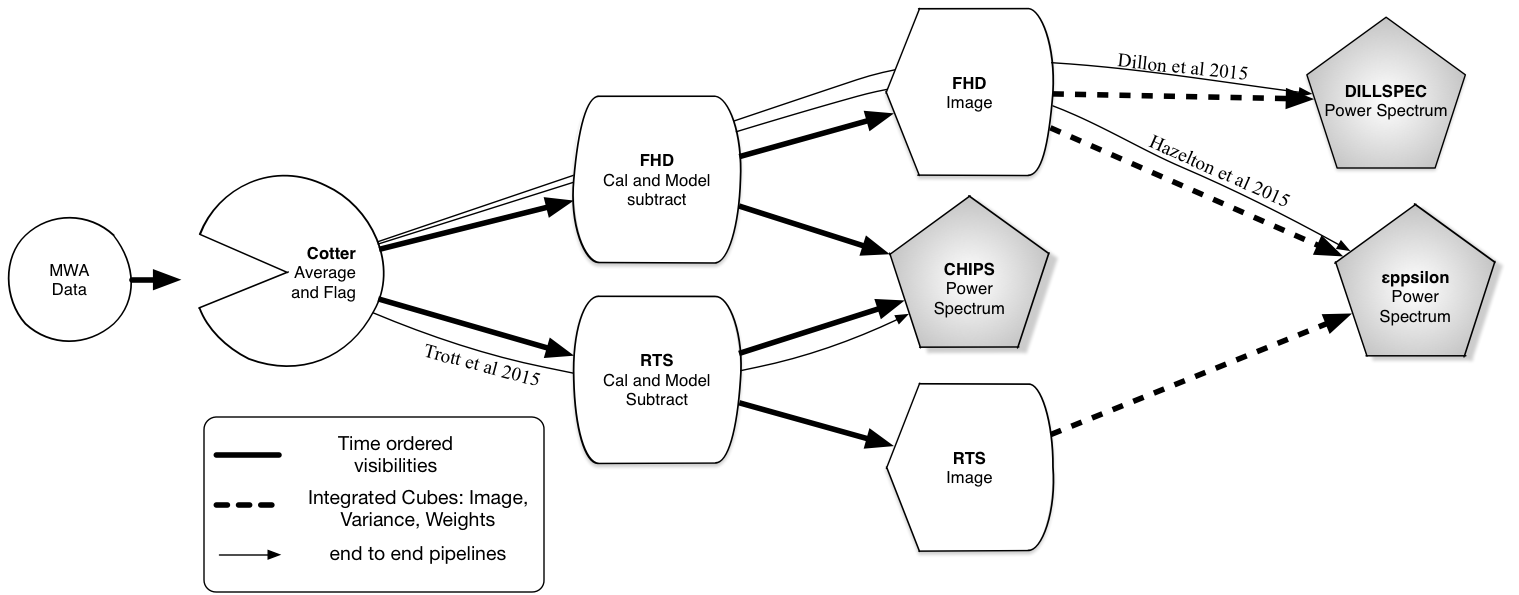
\includegraphics[width=\textwidth]{figures/MWA_Pipes.png}
\caption{Parallel pipelines with cross-connections after foreground subtraction and imaging are compared against each other as a guard against error.  Cotter uses AOFlagger to flag RFI and averages by a factor of 8. The averaged snapshots are passed to either FHD or RTS for calibration and imaging, EPPSILON takes the resulting snapshots, averages them in LST and estimates the power spectrum. CHIPS taps into the RTS and FHD to get calibrated and foreground subtracted time-ordered (not yet gridded) visibilities which it then uses to make its own estimate of the power spectrum. }
\label{fig:pipes}
\end{center}
\end{figure*}

\subsection{Calibration and Imager \#1: RTS}
\label{sec:RTS}
The MWA Real Time System (RTS) is a radio interferometry software package specifically written to calibrate and image MWA data \citep[][Mitchell et al. in prep]{Ord:2010p7534}. The RTS incorporates algorithms intended to address a number of known challenges inherent to processing MWA data, including; wide-field imaging effects, direction-dependant (DD) antenna gains and polarization response, and ionospheric refraction of low-frequency radio waves. Each MWA observation (112s) is processed through a separate instance of the RTS. The RTS is also parallelised over frequency so that each coarse channel (32 * 40 kHz fine channels) is processed largely independently of the other coarse channels, with only information about the measured ionospheric offsets communicated between processing nodes.  Calibration and model subtraction were based on the TBD catalog. 

The RTS calibration strategy is based upon the 'Peeling' technique proposed by \cite{Noordam:2004p2379}. The brightest (apparent) radio sources in the field of view are sequentially and iteratively processed through a Calibrator Measurement Loop (CML). During each pass through the CML; i) the expected (model) visibilities of known catalogue sources are subtracted from the observed visibilities. For the data processed in this work, TBD sources are subtracted for each observation. ii) The model visibilites for the targeted source are added back in and phased to the catalog source location. Any ionospheric offset of the source can now be measured by fitting a phase ramp to the phased visibilities. iii) The strongest sources are now used to update the direction-dependant antenna gain terms, while weaker sources are only corrected for ionospheric offsets. For this work, TBD sources are used as full DD calibrators and TBD sources are set as ionospheric calibrators. The CML is repeated until the gain and ionospheric fits converge to stable values. The TDB strongest sources are then subtracted from the calibrated visibilities and the residuals are passed to the visibility-based power spectrum described in Section \ref{sec:CHIPS} and shown in Figure \ref{fig:pspec_compare}.  A single bandpass for each tile is found by fitting a 2nd order polynomial to each coarse channel. Calibration and model subtraction parameters are summarized in Table \ref{tab:cal_sub_parms}. %how much flux is subtracted in total?

The RTS uses a snapshot imaging approach to correct for wide-field and direction-dependant polarization effects. Following calibration, the residual visibilities are first gridded to form instrumental polarization images which are co-planar with the array. These images are then regridded into the HEALPIX frame with wide-field corrections and conversion to Stokes applied through the regridding weights. It is also possible to use the fitted ionospheric calibrator offsets to apply a correction for ionospheric effects across the field during the regridding step, but in this work this correction has not been applied. See \citet{Clark_Allen_Arcus_et_al__2010} for a more complete description of the RTS imaging algorithms.  The resulting image spectral cubes, output on a 112s cadence paired with a spectral image cube of the point-spread function (Fourier dual to the weights in the $uvf$ plane), and the variance (dual to the $uvf$ weights squared).  The mean of the image cube is shown in Figure \ref{fig:image_compare}.
\begin{deluxetable}{lcr}
\tablecolumns{3}
\tablecaption{MWA EoR Calibration and Model subtraction Parameters }
\tablehead{
\colhead{parameter}  & 
\colhead{value} &
\colhead{free parameters}
}
\startdata
&RTS&\tabularnewline
\hline
passband & 2nd order poly per coarse channel & 48 per tile  \tabularnewline
gain & amplitude and phase & 2 per tile \tabularnewline
Direction Dependent & 2x2 Jones matrix & 4 per DD source  \tabularnewline
Catalog &TBD& \tabularnewline
Number of sources subtracted & TBD& TBD flux cut\tabularnewline 
\tabularnewline
& FHD & \tabularnewline
\hline
passband & fine channel gain spectrum & 768 channels for entire array \tabularnewline
passband & 2nd order poly over full band (1st order for phase) & 3 per tile\tabularnewline
gain & amplitude and phase & 2 per tile\tabularnewline
Catalog &TBD& \tabularnewline
Number of sources subtracted & TBD&TBD flux cut\tabularnewline 
\enddata
\label{tab:cal_sub_parms}
\end{deluxetable}

\subsection{Imager \#2: FHD}
Fast Holographic Deconvolution (FHD, \cite{Sullivan:2012p9457}) is a calibration and imaging algorithm designed for very wide field of view interferometers with direction- and antenna-dependent beam patterns. FHD has particularly been designed with a focus on producing an accurate measurement of the power spectrum complete with proper error propagation. Like the RTS, FHD uses the  beam pattern for gridding visibilities to the u-v plane, and its Hermitian conjugate for de-gridding simulations to form model visibilities. The  beam model is composed of the measured antenna response to the electric field for each antenna element and at every fine frequency channel, convolved with the response of the second antenna that forms the visibility. Three data outputs are necessary from gridding in order to calculate the image based power spectrum with accurate error bars: the measured visibilities, gridded with the  beam model\footnote{Note that the resulting image will be tapered by the average primary beam squared}; the weights, obtained by gridding the  beam model; and the variance, obtained by gridding the squared beam model.

The FHD calibration and imaging pipeline both measures and removes foregrounds. In the first mode, we deconvolve a deep observation with XXX hours on each field (a small fraction of the total data) to generate a high quality map of the foregrounds. This foreground model includes both compact and extended sources and diffuse structure such as the galaxy, and it is used as an input to the second FHD imaging mode. In the second mode we process all 1000 hours of EoR observations, but do not perform any deconvolution. Instead, we generate model visibilities using the full polarized direction-dependent antenna gains, and calculate the on-field direction-independent calibration solutions for each 112s EoR snapshot. The residual visibilities formed by subtracting the calibration model from the data are first saved and sent to the visibility-based power spectrum pipeline (section XXX), and then gridded (again using the polarized primary beam) along with the weights and variance for the image-based power spectrum pipeline (section XXX). The snapshot image, weights, and variance cubes are Fourier transformed into the image domain. Deep integrations are produced by gridding all of these products into single HEALPix maps.


\begin{figure*}[h!]
\begin{center}
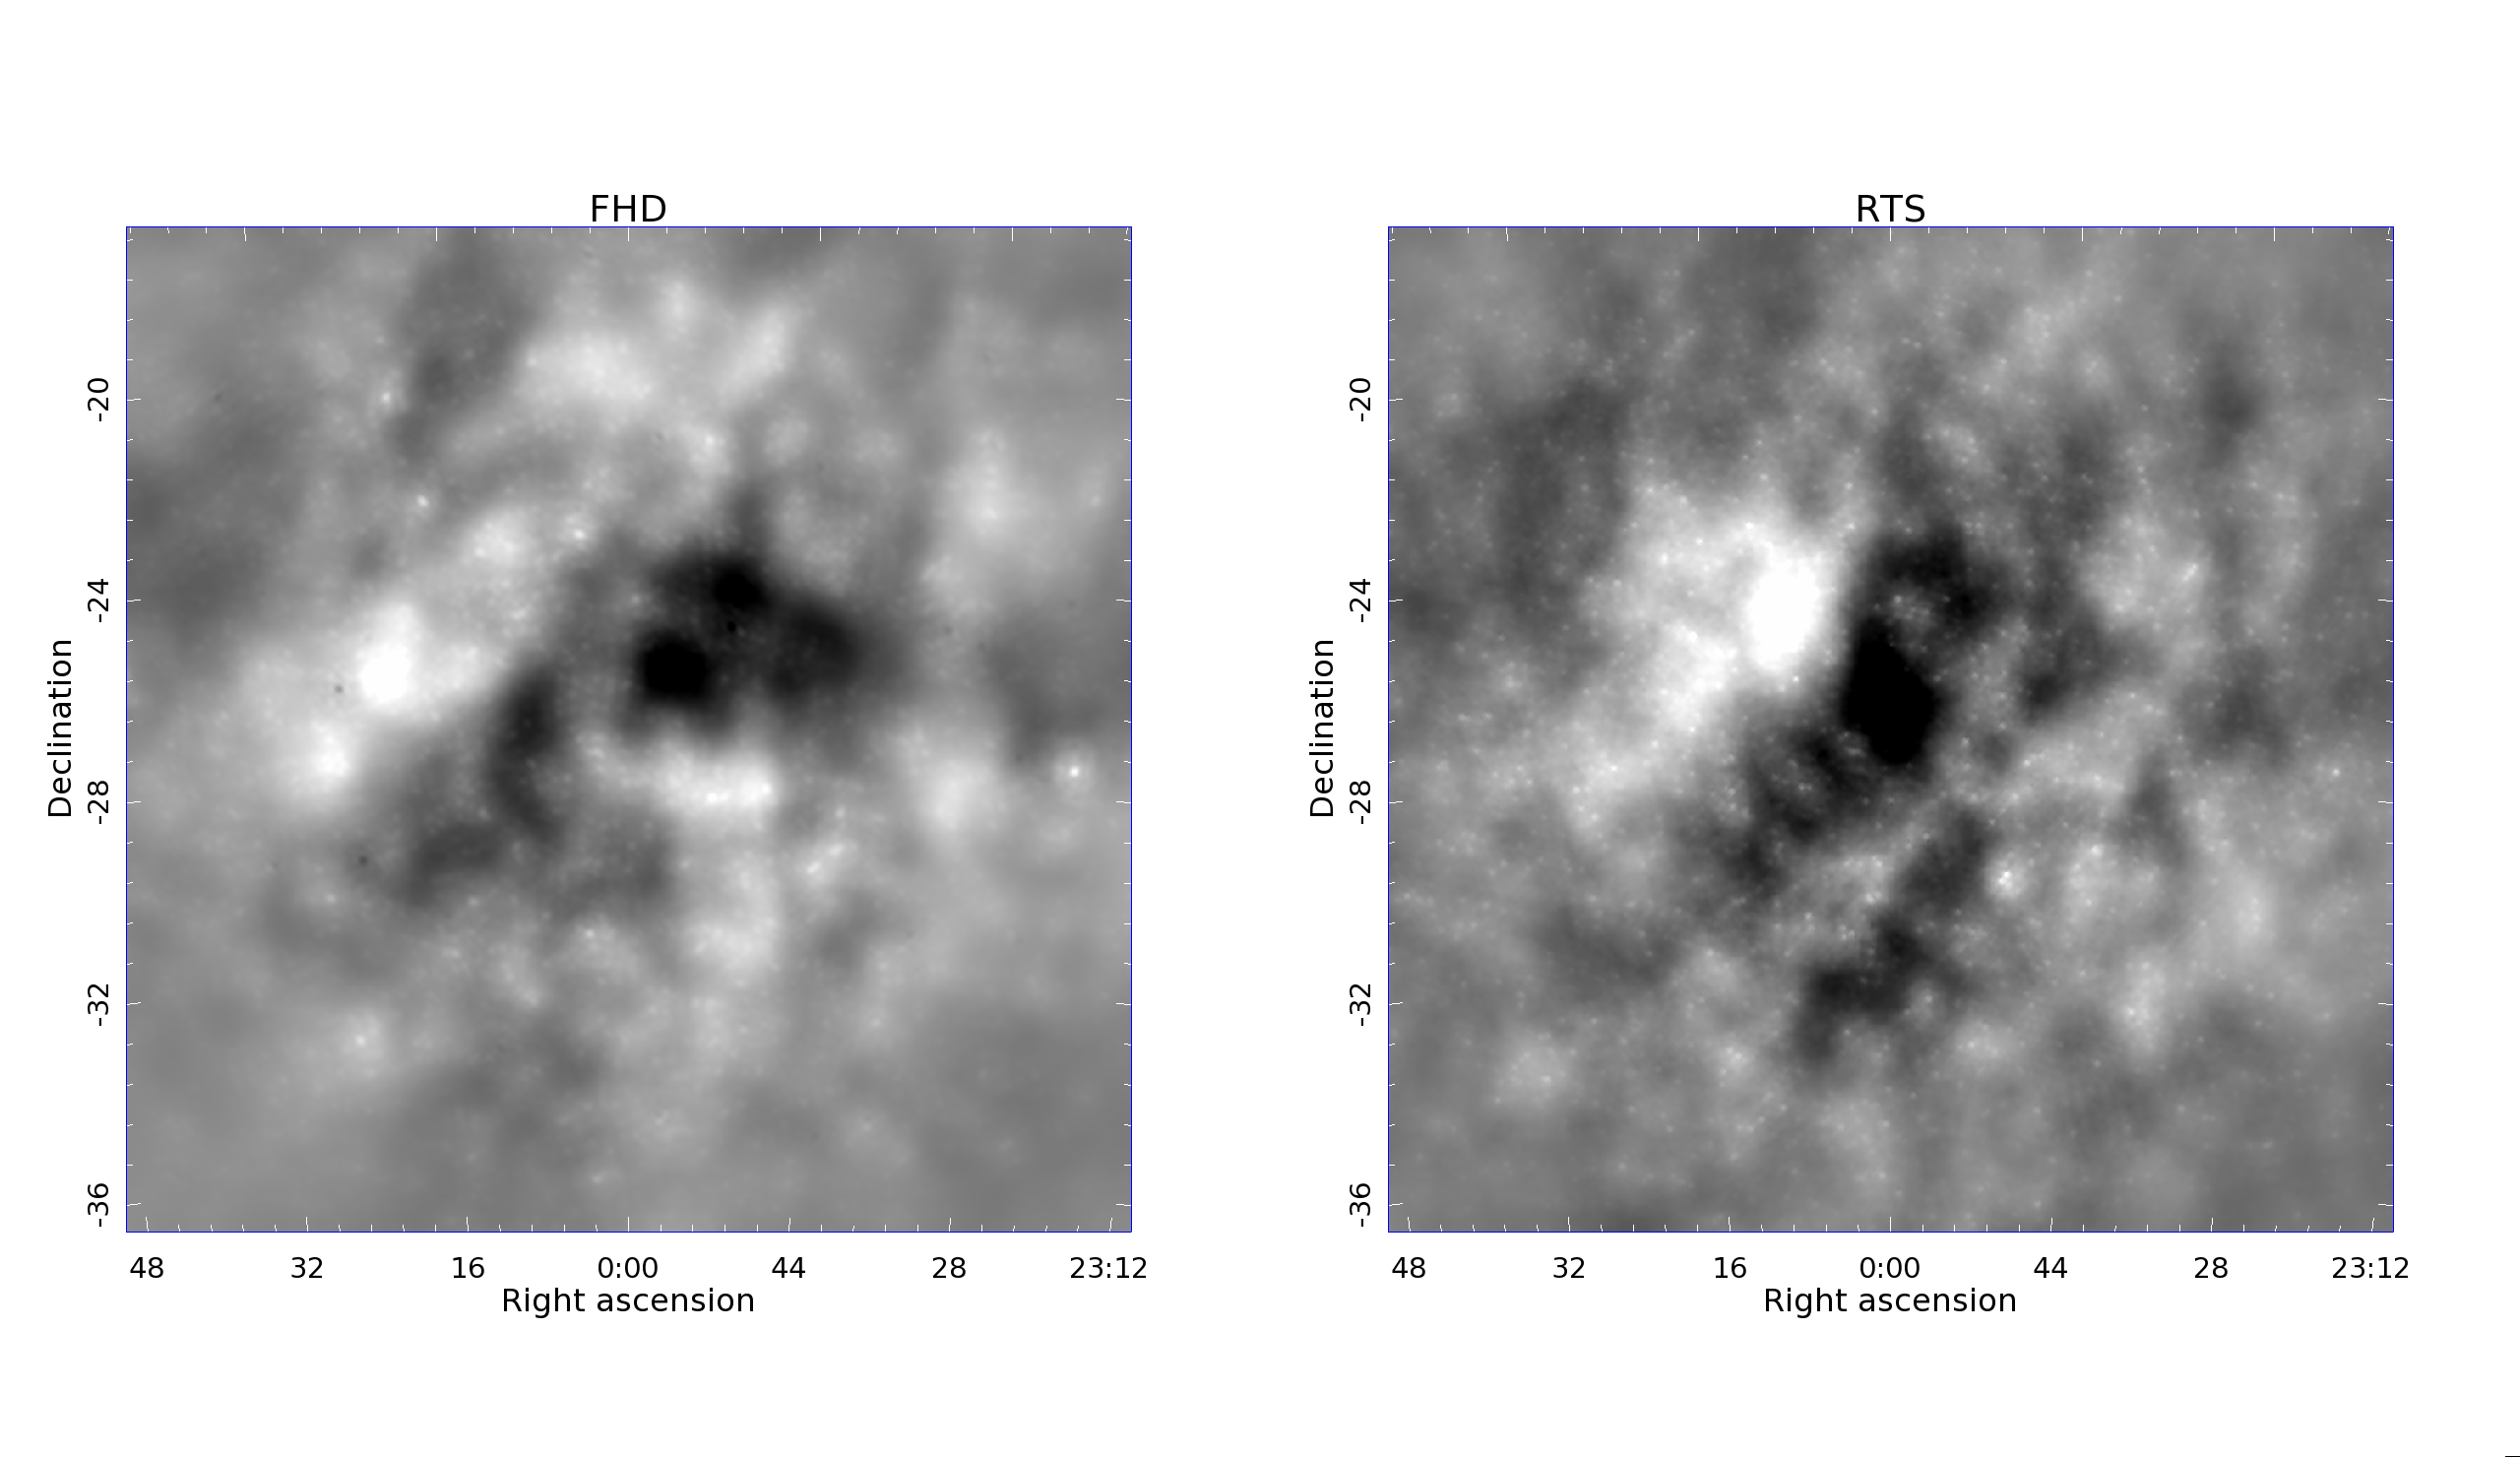
\includegraphics[width=0.9\textwidth]{figures/image_compare/image_compare.png}
\caption{Images from RTS and FHD.. \label{fig:image_compare}}
\end{center}
\end{figure*}

\subsection{Power Spectrum \#1: Image-based}
\label{sec:EPPSILON}
The direct propagation power spectrum method calculates a straight-forward power spectrum estimate and directly propagates the error bars through the full analysis. It requires pairs of holographically gridded image cubes in which the data has been split into interleaved time samples (referred to as even and odd cubes) along with matched cubes containing the weights and the variances [Do we want to add equations to describe these?].  The data, weight and variance cubes are Fourier transformed in two dimensions to take them to $uvf$ space where the covariance matrix is assumed in this method to be diagonal\footnote{Note that this is a better assumption if the $uv$ pixel size is well matched to the primary beam size}. The data (variance) cubes are then divided by the weight cubes (weight cubes squared) to arrive at the best estimates of the sky and variances. Next the sum and difference of the even and odd cubes are computed with variances given by adding the reciprocal of the even and odd variances in quadrature. The difference cube then contains only noise (as long as the time interleaving is fine enough) and the sum cube contains both sky signal and noise.

The next step is to apply a spectral window function (typically a Blackman-Harris) and to Fourier transform in the frequency direction. The covariance matrix (diagonal in $uvf$; terms given by the sum and difference variances) is propagated through this Fourier transform and covariances between non-identical modes are marginalized over. This results in a two-by-two covariance matrix for each Fourier mode containing the $cos^2$ and $sin^2$ terms on the diagonal and the $cos\times sin$ cross term in the off-diagonal elements. These covariance matrices (and the associated data) are then diagonalized for each Fourier mode (as in Lomb (1976) [N.R. Lomb, Astrophysics and Space Science, vol 39, pp. 447-462, 1976] \& Scargle (1982) [J.D. Scargle, The Astrophysical Journal, vol 263, pp. 835-853, 1982]), producing two terms that are squared and combined to get the best power estimates. The sky signal power is best estimated by the square of the sum cube minus the square of the difference cube\footnote{This is mathematically identical to the even/odd cross power if the even and odd variances are identical} while the square of the difference cube provides a realization of the noise in the power spectrum. Finally the power cubes can be averaged (using a variance weighting) in $k_x-k_y$ rings to get to a two dimensional $k_{\|}-k_{\bot}$ space.

\subsection{Power Spectrum \#2: Visibility-based}
\label{sec:CHIPS}
The second power spectrum estimation method computes the maximum likelihood estimate of the 21~cm power, using residual visibilities from the RTS and FHD. It aims to extract maximal information about the signal of interest by incorporating maximal information about the instrument and foreground signals by correctly characterizing the statistical properties of the data. The approach is similar to that used by Liu \& Tegmark (2011)[http://dx.doi.org/10.1103/physrevd.83.103006], but with the key difference of being performed entirely in $uv$-space, where the data covariance matrix is simpler (block diagonal), and feasible to invert. This approach also allows straightforward estimation of the variances and covariances between sky modes by direct propagation of errors, and operates entirely within $uv$-space with complex-valued calibrated and peeled visibilities.

The method involves four major steps: (1) Grid and weight measured visibilities onto the $uv$-plane using the primary beam model, and combine all data into $w$-stacks, for each spectral channel; (2) compute the least squares spectral (LSS) transform along the frequency dimension to obtain the best estimate of the line-of-sight spatial sky modes (this technique is comparable to that used in the image-based pipeline, described above); (3) compute the maximum-likelihood estimate of the cross-power spectrum, incorporating foregrounds and radiometric noise, by averaging $k_x$ and $k_y$ modes into annular modes on the sky, $k_\bot$; (4) compute the uncertainties and covariances between power estimates. The first step is the most computationally-intensive, requiring processing of all the measured data. It also includes a step to account for the spectral smearing of the sky information that occurs when observed through the instruments primary beam. This accounting aims to connect the information available from the sky with the information in the data. Unlike the image-based power spectrum method described above, the visibility-based pipeline uses a finely-sampled $uv$-plane to correctly characterise the smearing due to the primary beam.

The line-of-sight transform is performed once, and the uncertainties propagated. The final two steps in the pipeline are performed on the final full set of beam-weighted and transformed visibilities. These steps can be performed multiple times using different foreground models, and are also applied iteratively to converge to the maximum likelihood solution. The resulting dataset provides an estimate of the power in each $k_\bot,k_\parallel$ mode, and the variances and covariances associated with these estimates.

A two paragraph description of how the power spectrum is estimated from residual visibilities.  How are error bars estimated (the math part). But also the operational part, which axes are multiplied, which are averaged etc.  



\section{Results}
We compare images and power spectra, cross-checking at the half-way point.

\subsection{Images}
Comparing the images (figure) and fluxes (figure). 

The output of a deep imaging run is a foreground model which can be subtracted from the rest of the data. Both imagers seem to agree on the structure of the sky and the fluxes of the sources.

Agree on set of obsids: Bart/Adam
select/generate/send to Danny FHD fits images: Adam ToDo  
select/generate/send to Danny RTS fits images: Bart ToDo  
flux flux comparison: Patti with help from Danny




\subsection{Power Spectra}
We've got four power spectra (figure). The two "main" pipelines, and the cross-checks. They look more or less the same. Some of the differences stem from operational limitations on the total bandwidth produced by the RTS (in the process of being increased) and the amount of time averaging done.  

Power spectra (same obses as images)
Cath Todo
Bryna Todo

\begin{figure*}[h!]
\begin{center}
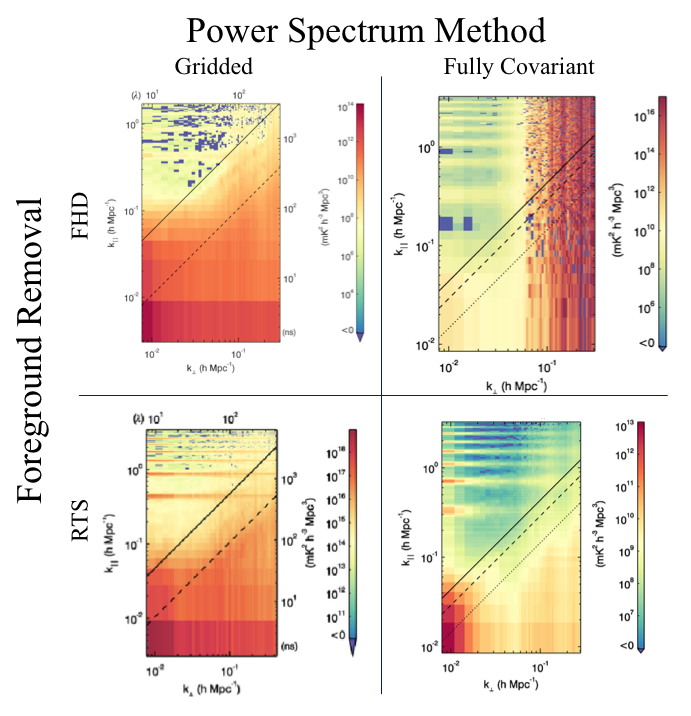
\includegraphics[width=0.8\textwidth]{figures/MWA_PS_compare1/MWA_PS_compare.png}
\caption{MWA power spectra computed using two foreground subtraction methods and two power spectrum estimation methods.  In the top row data have been calibrated to a catalog followed by subtraction of a deeper catalog modelled into instrumental space using the Fast Holographic Deconvolution method, in the bottom row calibration and foreground subtraction have been performed with the MWA Real Time System.  In the left column, power spectra have been estimated with data that have had baselines averaged into a $uvf$ grid while in the right baselines are cross multiplied individually to make a optimally weighted estimate of the power spectrum.\label{fig:pspec_compare}}
\end{center}
\end{figure*}

\section{Conclusion}
images are the same, power spectra are very similar.
Other Things people will want to know that I haven't put in yet. Tsys. RFI. How do the fluxes compare with catalogs? How deep is the power spectrum?.

\bibliography{bibliography/library.bib}

\end{document}

